\section{提案手法}
\label{section_method}
\subsection{シミュレーションの概要}
シミュレーションの概要を図\ref{fig_simulation}に示す.

シミュレーションは,汎用エージェントモデリング・シミュレーションプラットフォームであるGAMA上で行う.

シミュレーション結果,すなわち,公共交通機関の混雑度は,GAMAの地図上でリアルタイムに可視化する.

対象とするフィールドは,京都エリアの一部地域とする.対象地域については,ランドマークや人の分布を分析した後に決定する.

\begin{figure}[H]
  \begin{center}
    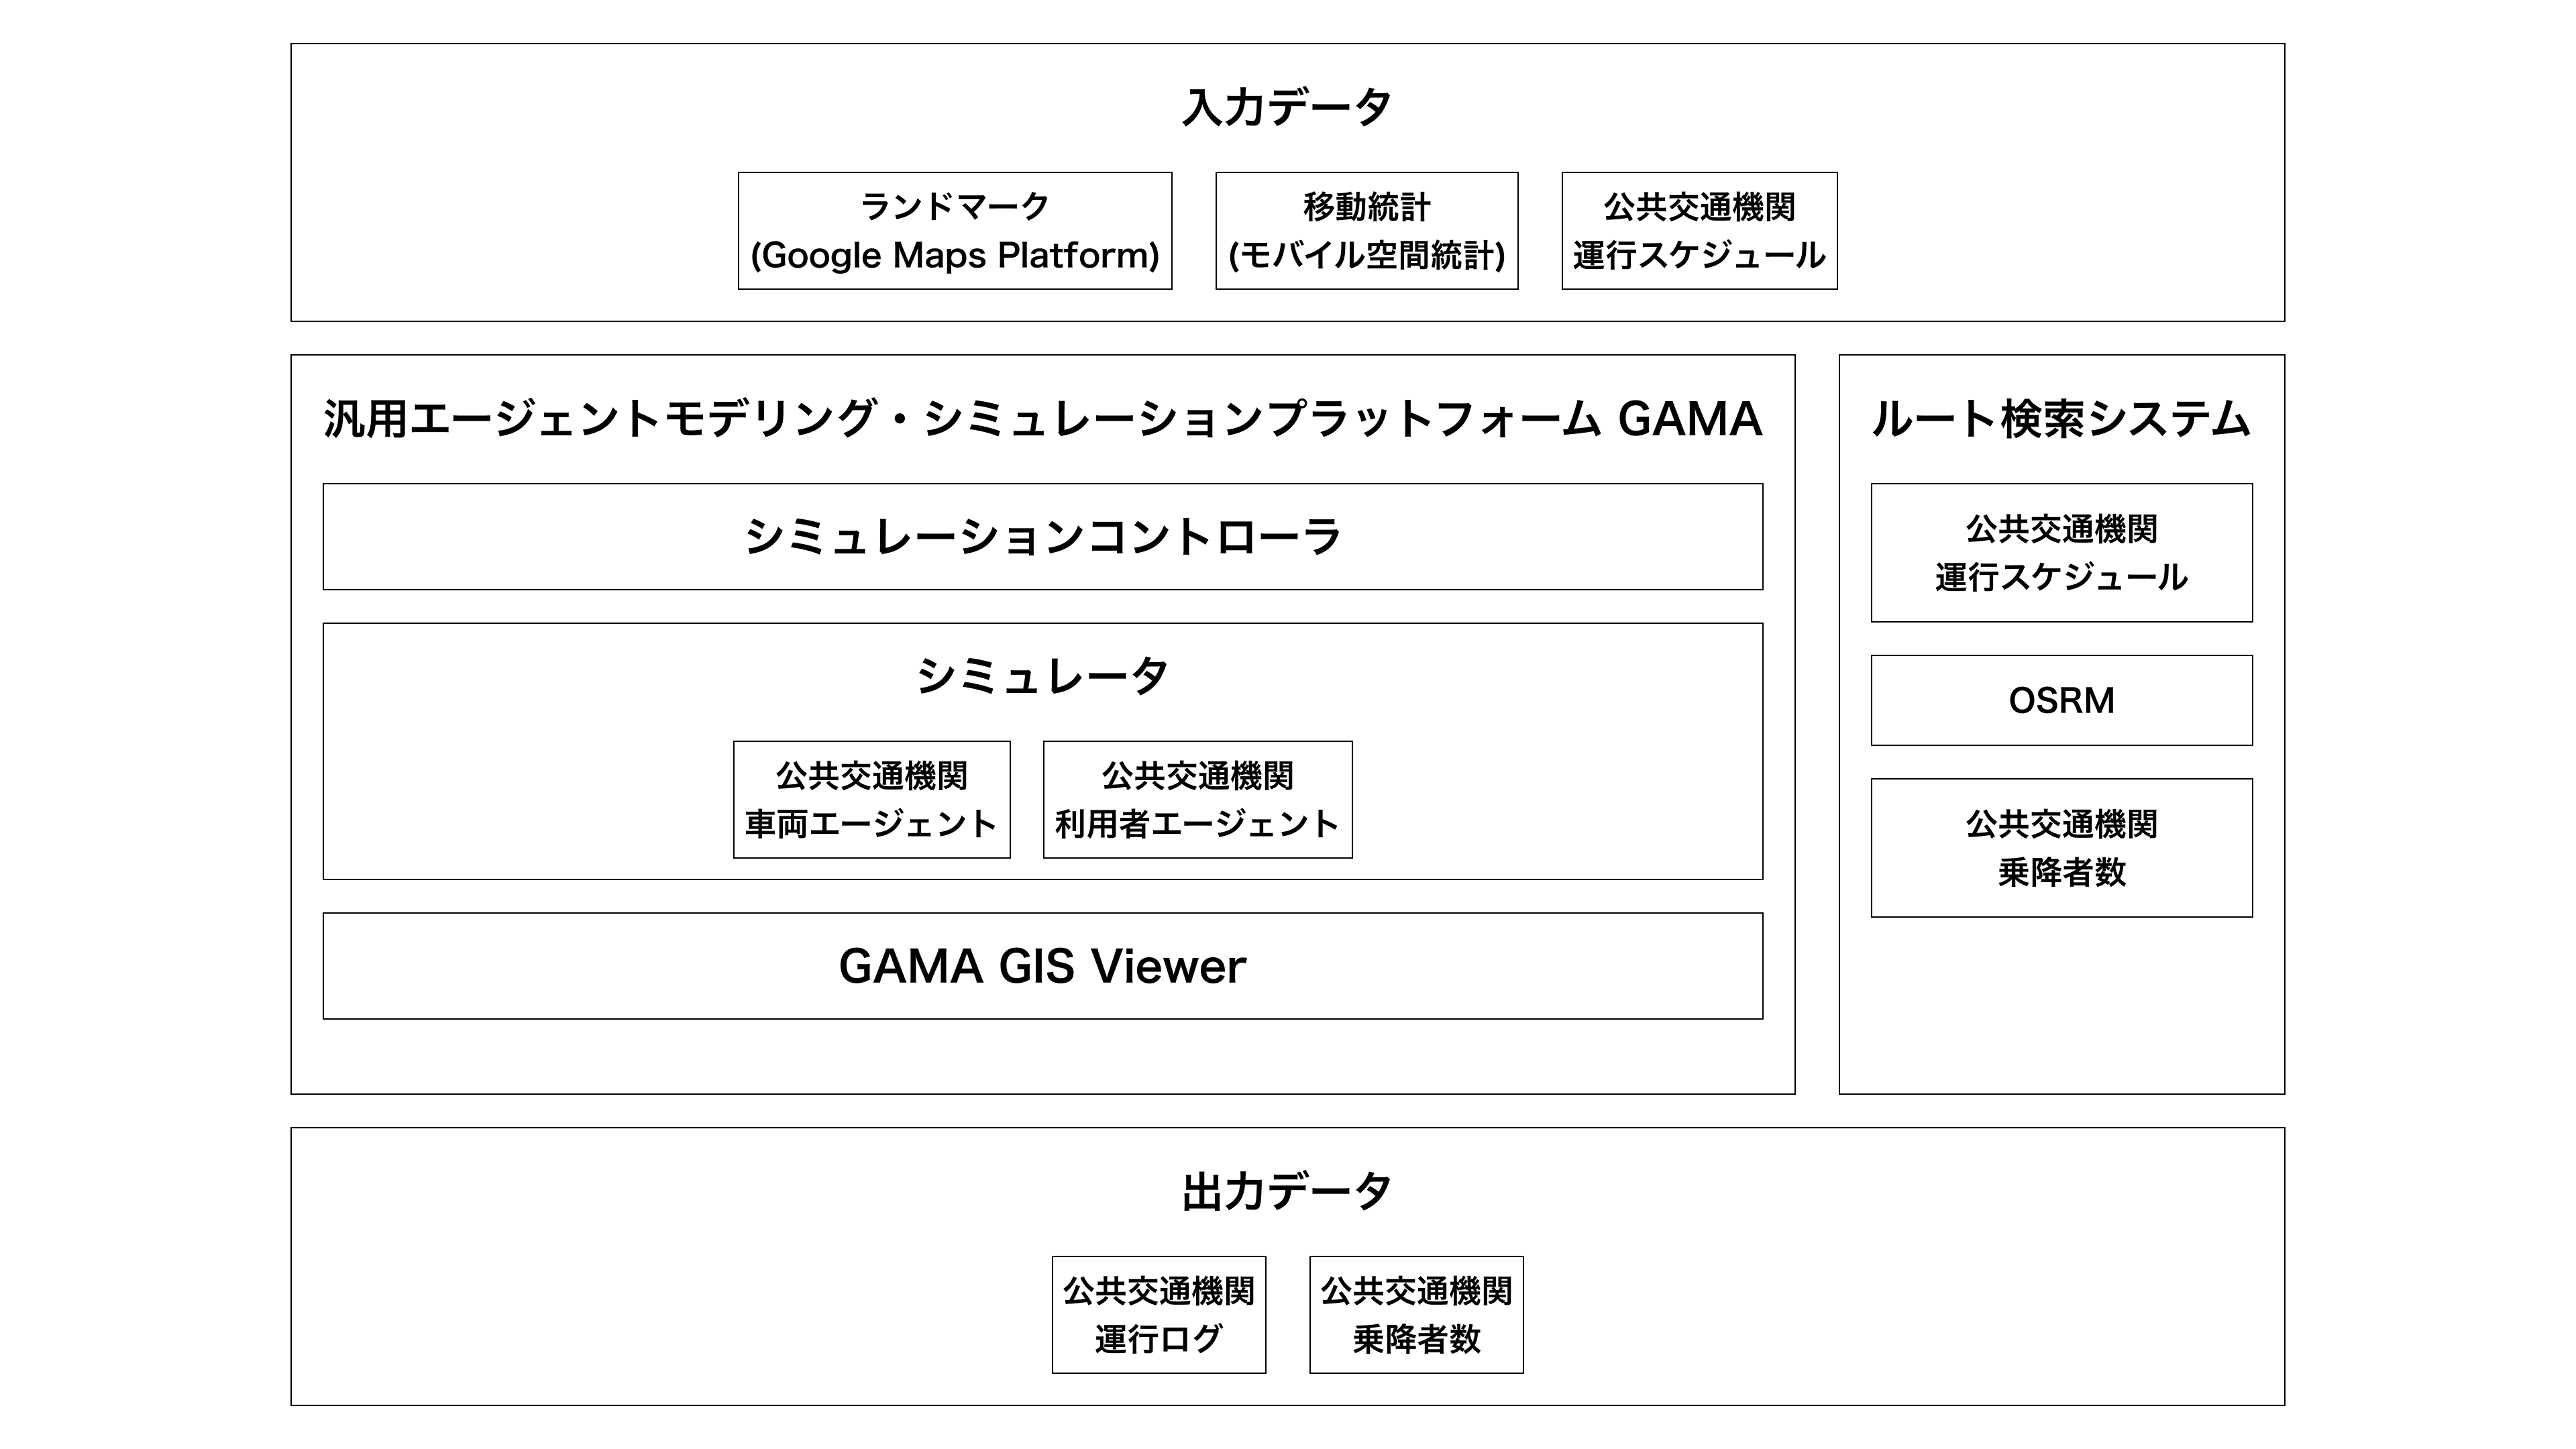
\includegraphics[width=1.0\linewidth]{assets/simulation_summary.png}
    \caption{シミュレーションの概要}
    \label{fig_simulation}
  \end{center}
\end{figure}

\subsection{公共交通機関利用者エージェントの定義}
\label{section_agent}
図\ref{fig_simulation}に示したシミュレーションにおいて,シミュレータの公共交通機関利用者エージェントの定義の詳細を以下に示す.

エージェントの単位は,公共交通機関利用者一人一人とする.

エージェントの内部状態は,以下の要素から構成される.
\begin{itemize}
  \item 拠点
  \item 目的地
  \item 目的地までのルート (時間,公共交通機関の情報を含む)
  \item 満足度 (移動にかかる時間,料金,混雑度から計算)
  \item 現在地
\end{itemize}

拠点は,住民の場合は自宅,旅行者の場合は宿泊先とする.

エージェントは,以下の情報を取得することができる.
\begin{itemize}
  \item ランドマークのリスト
  \item 目的地までのルート候補
    \begin{itemize}
      \item 出発・到着時刻
      \item 所要時間
      \item 料金
      \item 混雑度
    \end{itemize}
\end{itemize}

エージェントは,以下のアクションをとることができる.
\begin{itemize}
  \item 目的地の決定・変更
  \item ルートの選択・変更
  \item 移動
\end{itemize}

さらに,エージェントは,以下の意思決定機構を持つ.
\begin{itemize}
  \item 目的地決定
  \item ルート選択
\end{itemize}

目的地決定機構では,\ref{section_mobaku}節で取り上げるモバイル空間統計のデータから,住民,旅行者それぞれの移動の特徴を分析し,その傾向から機構を決定する.

ルート選択機構では,移動にかかる時間,料金,混雑度などを鑑み,満足度が最も高くなるようなルートを選択する.

\subsection{データ}
\subsubsection{Google Maps Platform}
Google Maps Platform\footnote{https://mapsplatform.google.com}は,Googleが提供する地図情報を利用するためのAPI群である.本研究では,Google Maps PlatformのAPIを利用して,観光スポットや住民が日常的に利用する施設等のランドマーク情報を取得する.

\subsubsection{モバイル空間統計}
\label{section_mobaku}
モバイル空間統計\footnote{https://mobaku.jp}は,NTTドコモが提供するサービスである.NTTドコモのモバイル端末から収集された位置情報を元に,人々の移動パターンを分析することができる.本研究では,モバイル空間統計のデータを利用して,季節や曜日に注目した,住民と旅行者の移動パターンを分析する.

モバイル空間統計は,いくつかの種類の統計情報を含んでいる.本研究で利用を予定している統計情報を以下に示す.

\begin{itemize}
  \item 分布統計 (国内居住者)
  \item 国内旅行者動態統計 (国内居住者)
  \item 人口流動統計
\end{itemize}

\subsubsection{公共交通機関運行スケジュール}
公共交通機関運行スケジュールは,General Transit Feed Specification\footnote{https://gtfs.org} (GTFS) というオープンフォーマットで公開されているオープンデータである.本研究では,エージェントが移動に使用する公共交通機関の路線や時間の選択肢として使用する.
